\blankpage

\thispagestyle{empty}
\clearpage
\begin{tikzpicture}[remember picture, overlay]
\node at (3,-7) {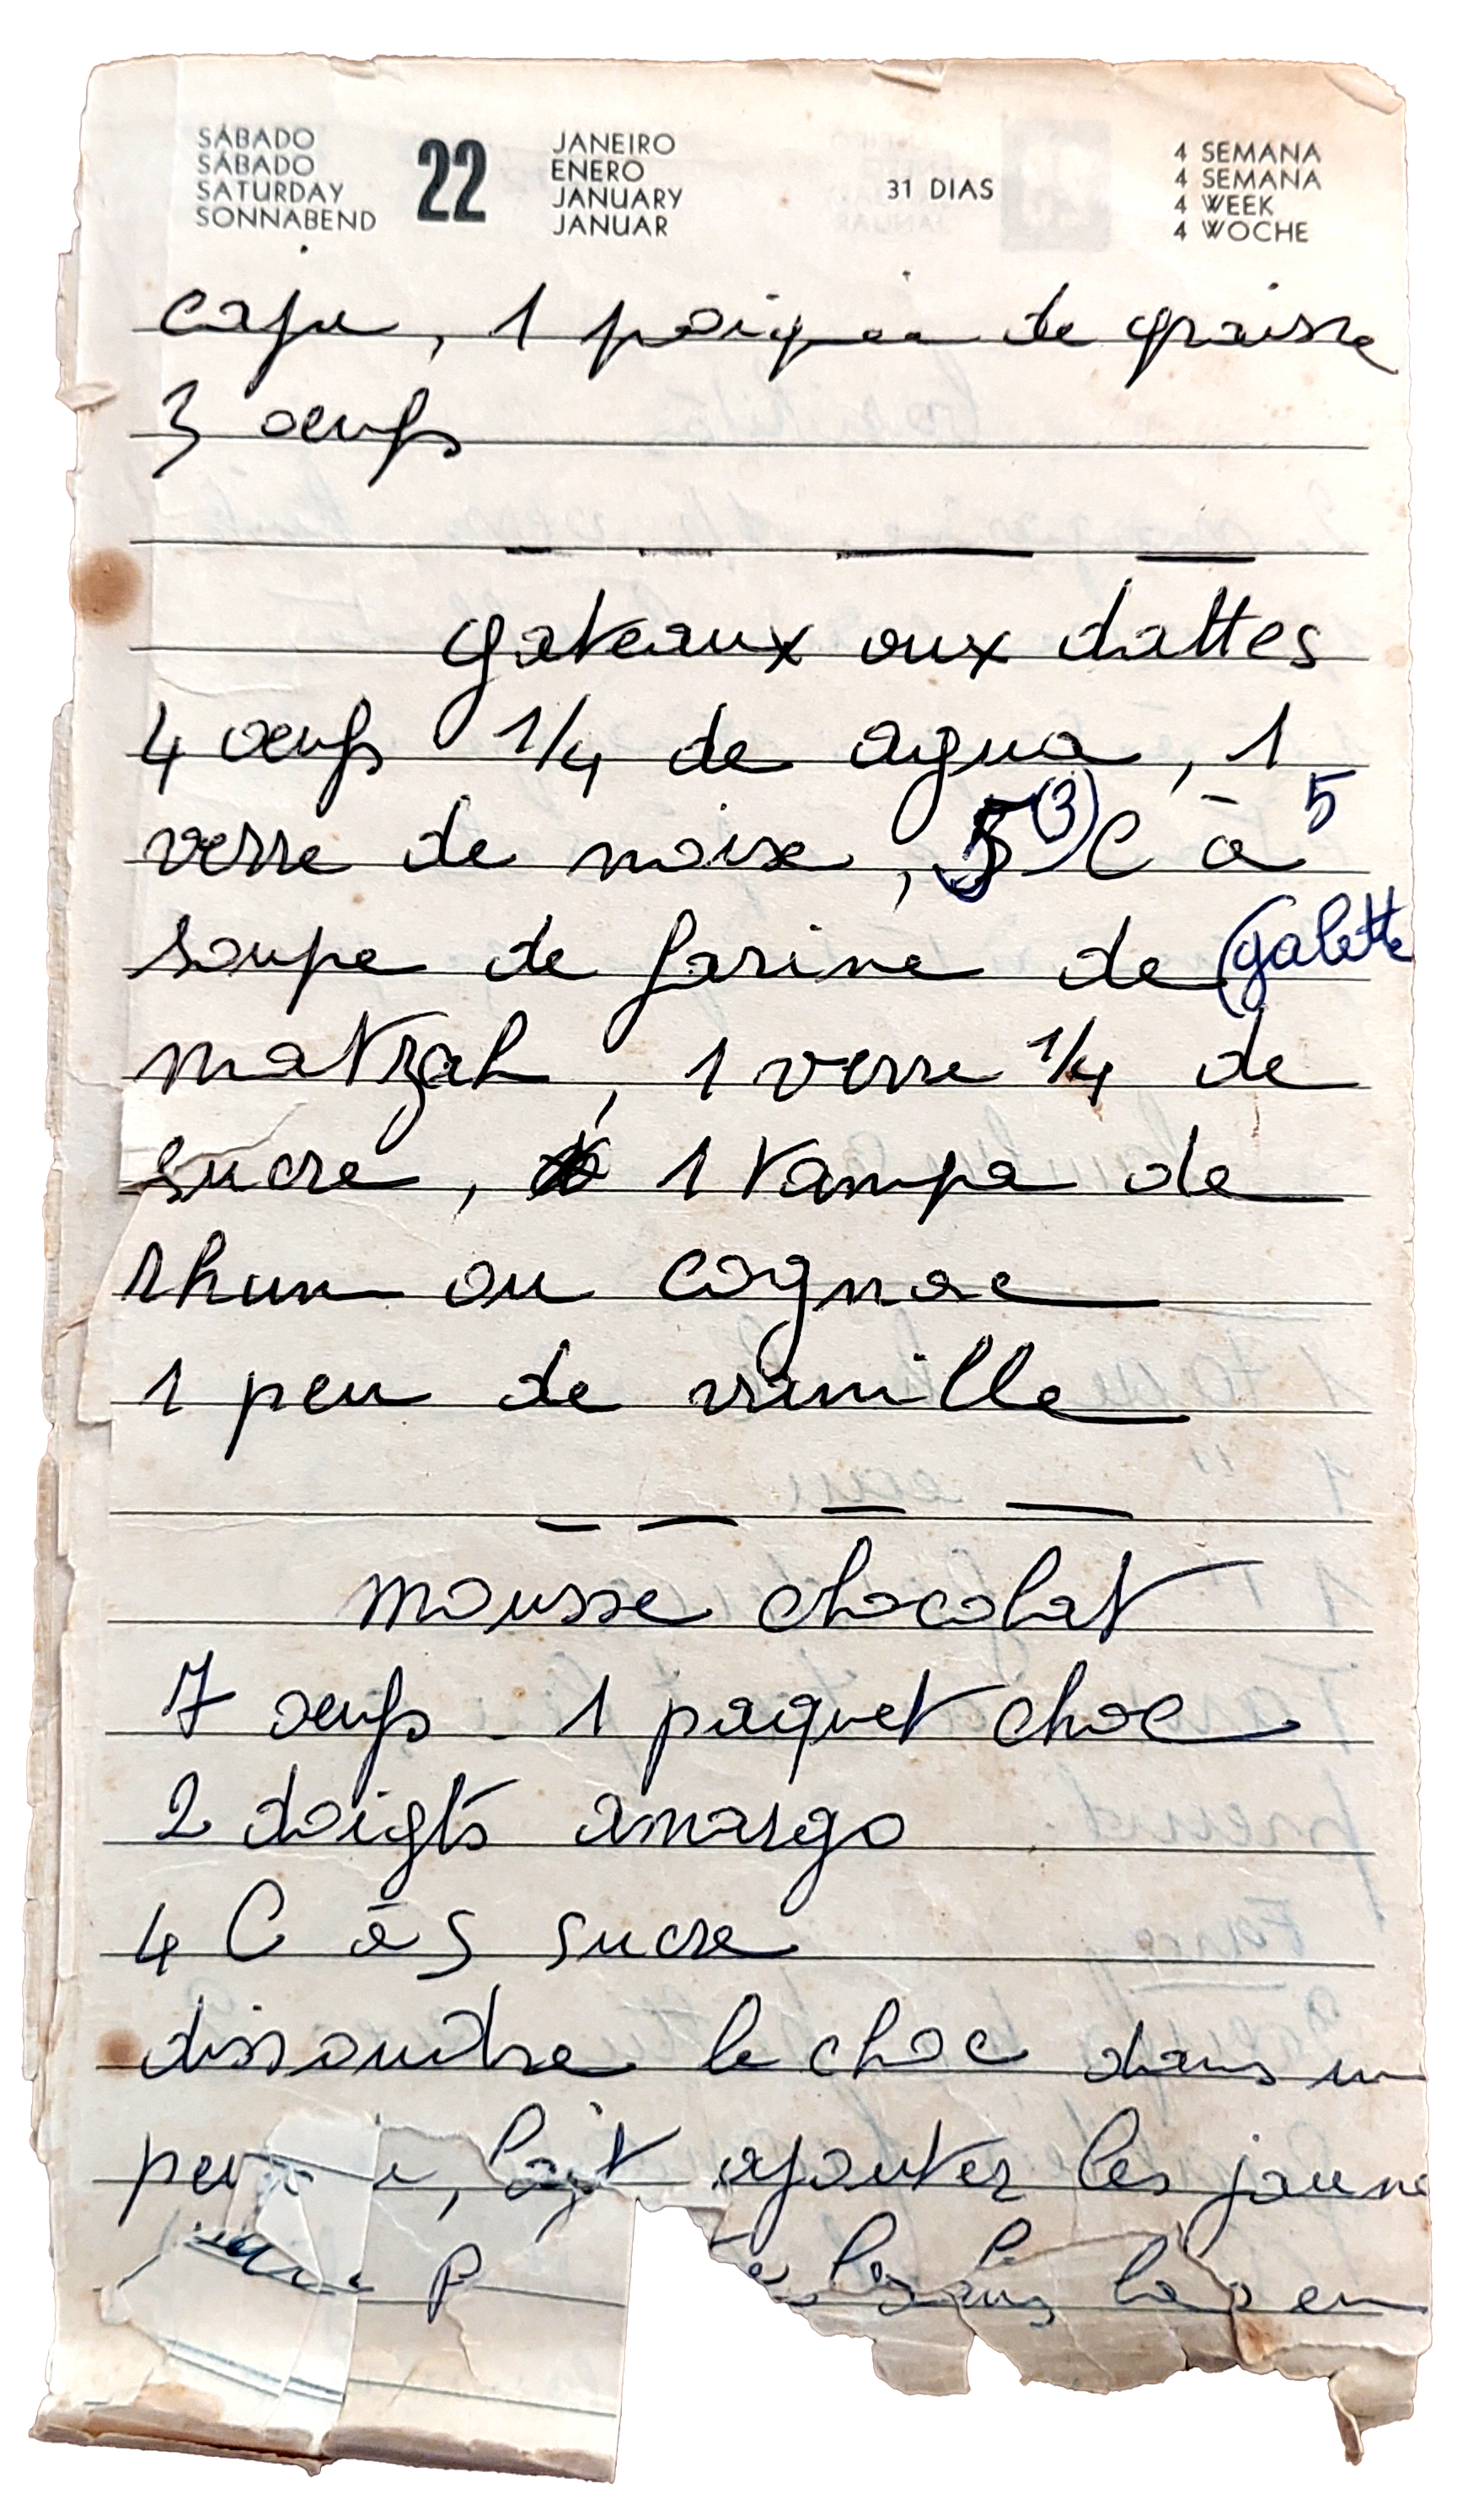
\includegraphics[width=8cm]{./recettes/edités/Gateau aux dattes et Mousse chocolat.jpg}}; 
\end{tikzpicture}\clearpage\thispagestyle{empty}
% \begin{tikzpicture}[remember picture,overlay]
% \fill[black] (-3,3.5) rectangle (14,-21.5);
% \end{tikzpicture}
\clearpage

\chapter*{Gâteau aux dattes}

\section{Ingrédients originaux}

\begin{itemize}
\item 4 œufs
\item 1 verre de noix
\item 5 c à soupe de farine de galette matzá
\item 1/4 verre de sucre
\item 1 tampo de rhum ou cognac
\item un peu de vanille
\end{itemize}

\section{Préparation adaptée}

Battez les œufs avec le sucre jusqu’à obtenir un mélange clair. Ajoutez le cognac et deux cuillères à soupe de vanille en mélangeant bien. Incorporez la farine de matsá, puis ajoutez les noix et les dattes hachées selon votre goût (si elles sont sèches, hydratez-les rapidement dans de l’eau tiède). Mélangez jusqu’à obtenir une pâte homogène, en ajustant la texture avec un peu de liquide si nécessaire ; versez dans un moule beurré et faites cuire au four préchauffé à 180°,\textsc{c} pendant environ 30 à 40 minutes, jusqu’à ce que le gâteau soit doré et ferme.

\chapter{Bolo de tâmaras}

\section{Ingredientes originais}

\begin{itemize}
\item 4 ovos
\item 1 copo de nozes
\item 5 colheres de sopa de farinha de matzá
\item 1/4 de copo de açúcar
\item 1 tampinha de rum ou conhaque
\item Um pouco de baunilha
\end{itemize}

\section{Modo de preparo adaptado}

Bata os ovos com o açúcar até obter uma mistura clara. Adicione o conhaque e duas colheres de sopa de baunilha, misturando bem. Incorpore a farinha de matzá e, em seguida, acrescente as nozes e as tâmaras picadas a gosto (se estiverem secas, hidrate rapidamente em água morna). Misture até obter uma massa homogênea, ajustando a textura com um pequeno pouco de líquido se necessário; despeje em uma forma untada e leve ao forno preaquecido a 180°\,\textsc{c} por cerca de 30 a 40 minutos, até dourar e firmar.